\subsection{Wire Wonders: The Trade-Off of Fewer Segments!}

\begin{tcolorbox}[colback=gray!10, colframe=black, title=E9B11] 

What is a disadvantage of decreasing the number of wire segments in an antenna model below 10 segments per half-wavelength? 

\begin{enumerate}[label=\Alph*.]
    \item Ground conductivity will not be accurately modeled
    \item The resulting design will favor radiation of harmonic energy
    \item \textbf{The computed feed point impedance may be incorrect}
    \item The antenna will become mechanically unstable
\end{enumerate} \end{tcolorbox}

\subsubsection{Conceptual Understanding}

To understand the implications of reducing the number of wire segments in an antenna model, it is essential to recognize the relationship between the model's fidelity and the accuracy of the computations that arise from it. In antenna modeling, wire segmentation is crucial for accurately simulating the physical properties of the antenna, including impedance and radiation patterns.

When the number of segments is decreased below 10 segments per half-wavelength, the antenna model tends to lose detail in representing the actual current distribution along the wire, which can result in inaccurate calculations of the feed point impedance.

\subsubsection{Feed Point Impedance}

The feed point impedance of an antenna is a vital parameter that affects its performance and efficiency. It is determined by the antenna's geometry, material properties, and the surrounding environment, among other factors. An incorrect modeling of the impedance can lead to issues such as poor impedance matching with the transmission line, resulting in reflection and loss of signal power.

To illustrate, let’s consider the example of a half-wave dipole antenna:

1. A half-wave dipole antenna has a total length of approximately 1 wavelength or \(\lambda\).
2. For an antenna modeled with sufficient segments, the current distribution can be accurately calculated.

If we denote:

\[
\lambda = \frac{c}{f}
\]

where \(c\) is the speed of light and \(f\) is the frequency of operation. If for a given frequency \(f\) we determine a length of the antenna and reduce the segments, the following steps apply:

3. Calculate the number of segments \(n\) for a half-wavelength:
   \[
   n = \frac{\lambda}{\Delta l}
   \]
   where \(\Delta l\) is the length of each segment.

4. If \(n < 10\), the approximation of the current distribution becomes poor.

This can lead to a mismatch in the actual impedance sensed by the feed line leading to possible signal degradation.

\subsubsection{Conclusion}

In conclusion, maintaining a sufficient number of wire segments is critical for assuring accurate computations regarding an antenna's feed point impedance. A lack of adequate segment representation can result in incorrect models, which can adversely affect antenna performance. Thus, while models with fewer segments may seem appealing for simplicity or reduced computation time, they can lead to significant inaccuracies that are detrimental to overall communication effectiveness.

\begin{center}
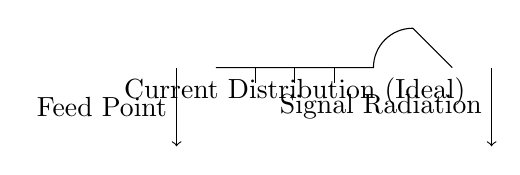
\begin{tikzpicture}
    \draw (0,0) -- (2,0) to[out=90,in=180] (2.5,0.5) -- (3,0);
    \foreach \x in {0.5, 1, 1.5} {
        \draw (\x,0) -- (\x,-0.2);
    }
    \node at (1,-0.3) {Current Distribution (Ideal)};
    \draw[->] (-0.5,0) -- (-0.5,-1) node[midway,left] {Feed Point};
    \draw[->] (3.5,0) -- (3.5,-1) node[midway,left] {Signal Radiation};
\end{tikzpicture}
\end{center}